\section{Introduction}
\label{sec:intro}

Language-model agents are increasingly proposed as operators of scientific experimentation:
selecting what to run, interpreting what comes back, and deciding what to run next
\citep{coscientist,chemcrow,szymanski2023autonomous}. The claim attached to this work is
that such agents will accelerate discovery in domains where experiments are the bottleneck.
Whether that claim holds is an empirical question, and answering it requires evaluating
agents under the conditions that make experimentation a bottleneck in the first place.

Existing evaluations cover important parts of this loop. BoxingGym limits an agent to ten
sequential queries and scores information gain and prediction; Olympus and Summit provide
executable optimization surfaces derived from chemistry; Minerva studies noisy parallel
batches under laboratory constraints; and budgeted and delayed-feedback Bayesian
optimization formalize cost or latency \citep{boxinggym,olympus,summit,minerva,
astudillo2021budgeted,verma2022delayed}. What remains difficult to measure is the combined
decision: allocating treatments to a tiered physical facility, interpreting the resulting
history, and issuing an operating recommendation while the experiments themselves incur
opportunity cost. A commercial tomato crop makes this combination concrete. It occupies a
greenhouse for seven months, block-level climate controls restrict which treatments can run
together, and a committed treatment cannot be revised after later evidence arrives.

\paragraph{\slowlab.} We introduce an executable benchmark for experimental design under
four conditions that hold at once. Feedback is \textbf{slow}: a cycle is $210$ days, and
the number of trials that run concurrently is capped --- unevenly, because some factors are
set for a whole block of units and others per unit, so replication and coverage compete for
the same physical resource. Observations are \textbf{noisy} enough that one unit does not
settle a question. Experimentation is \textbf{costly} in the objective's own units, since
testing a management regime means growing a crop under it and selling whatever results. And
a submitted design is \textbf{irreversible}: no branch, no checkpoint, no revert. Each
condition alone is familiar. Together they withdraw common forms of recourse, because an
agent can neither buy precision and coverage from the same units nor
find out which it needed before the season ends.

We validate this regime in controlled-environment horticulture. A published mechanistic
crop model \citep{jones1999reduced} supplies a traceable physiological basis, and an explicit
economic model puts recommendations and experimental opportunity cost in one currency,
net profit per square metre per day (\S\ref{sec:domain}). The published model does not make
benchmark difficulty author-independent: factor ranges, facility size, task budgets and
observation channels remain design choices and are reported as such. We distinguish three
roles throughout. A \emph{design policy} chooses which factor settings to test,
on how many units, and which physical units those are. Lamps and heating serve a whole
chamber while planting density and the pruning target are set per hydroponic loop, so an
allocation that varies temperature between two loops of one chamber describes an experiment
that cannot be performed. A \emph{history reader} turns the time-stamped evidence into a
recommendation. In a closed-loop LLM these two roles live in the same model, but we separate
them experimentally. The benchmark-side \emph{evaluator} scores their outputs using hidden
truth and never returns that information to the agent. Having committed, the agent may inspect measurements that are physically available as the
crop develops, but it cannot observe future yield or profit, revise the submitted treatment,
or release occupied capacity. After two or three cycles it must recommend. Figure~\ref{fig:overview}
shows the campaign loop.

\begin{figure}[t]
\centering
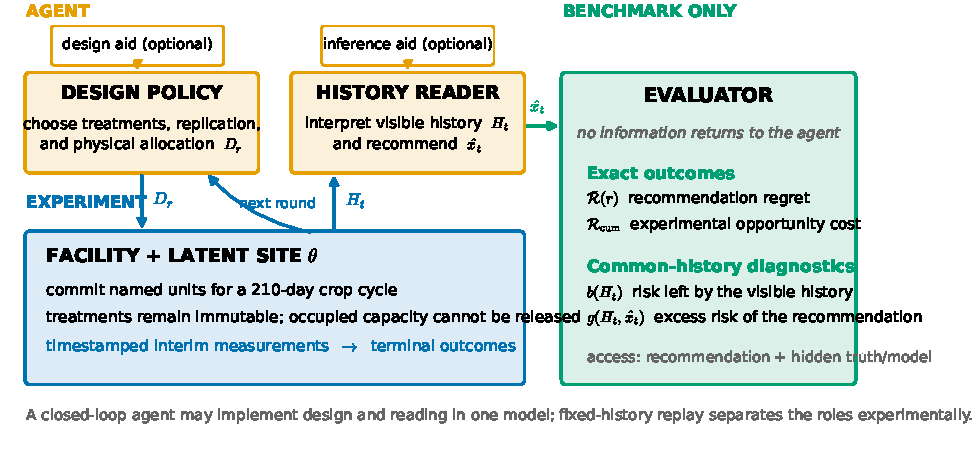
\includegraphics[width=\linewidth]{figures/fig0_overview.pdf}
\caption{\textbf{Roles and information flow.} The design policy commits treatments and
physical units; the history reader maps only the time-stamped visible history to a
recommendation. One closed-loop agent may implement both roles. The evaluator belongs to
the benchmark: it receives the recommendation and hidden truth to compute exact outcomes,
and uses the same visible history for diagnostic risks. It never supplies hidden information
to the agent. Interim observations can update the reader and the next design, but cannot
alter committed treatments or release occupied capacity.}
\label{fig:overview}
\end{figure}

Overall, our work makes the following contributions:
\begin{enumerate}[leftmargin=1.5em,itemsep=3pt,topsep=3pt]
  \item We formulate agent evaluation as three coupled capabilities in a resource-limited
    batch campaign: allocating treatments to feasible physical units, using the evidence
    revealed by the executed campaign, and issuing a final recommendation. The greenhouse
    instantiation enforces split-plot controls, finite capacity, economic accounting and
    time-appropriate inspection during a committed crop cycle.

  \item We define a common-history diagnostic. Bayes risk $b(H_t)$, recommendation risk and
    posterior excess $g(H_t,\hat x_t)$ condition on exactly the time-stamped history visible
    to the agent. Independent action-selection and evaluation samples prevent the evaluator
    from grading its own fitted action in sample.

  \item We separate design from history reading by replaying multiple readers on fixed
    executed histories, then test design and inference aids in frozen, site-paired
    protocols. The primary Luna and independent-site Sol results show no reliable final-
    regret improvement. A prospective same-site extension finds heterogeneous effects:
    inference is null for Luna, uncertain for DeepSeek V4.1 Flash, and beneficial for Qwen
    3.8 27B under the tested interfaces.
\end{enumerate}
